\chapter{Experiments and Results}
\label{chap:experiments-results}

\section{Introduction}

This chapter presents the experimental evidence used to answer the research
questions defined in Chapter~\ref{chapter:introduction}. The results are organised
in five parts: classifier baselines, generated-URL quality, controlled GAN
augmentation, external generalisation, and threshold selection. Browser
implementation and user evaluation are reserved for Chapter~7.

The primary comparisons use fixed real training identities, unchanged real
validation and test sets, and seeds 42, 43, and 44. Synthetic URLs are added
only to the training partition. Unless otherwise stated, percentage results are
the mean across the three seeds. Accuracy is reported for completeness, but it
is not interpreted alone because phishing prevalence varies substantially
between evaluation sets. Recall, precision, F1-score, ROC-AUC, FPR, and FNR are
considered together.

\section{Development Results from Versions 1 and 2}

Versions 1 and 2 established the first working baselines and exposed the main
experimental risk: high performance on a familiar random test split did not
guarantee equal performance on URLs collected from another source. Their
results are therefore retained as development evidence, but are not combined
statistically with Version~3 because the preprocessing, stored splits, and
evaluation protocols differ.

\begin{table}[htbp]
\centering
\caption{Summary of the first two experimental versions.}
\label{tab:v1-v2-summary}
\small
\begin{tabular}{@{}p{0.10\textwidth}p{0.22\textwidth}p{0.25\textwidth}p{0.33\textwidth}@{}}
\toprule
Version & Main real-data setting & Main internal result & Experimental lesson \\
\midrule
V1 & 2,568,184-row source file; 252,430-row internal test & LSTM F1 97.17\%; CNN F1 97.05\% & A large random split produced strong internal results, but did not establish source-independent generalisation. \\
V2 & Normalised frozen split: 2,055,821 train, 254,298 validation, 252,165 test & Three-seed mean F1: LSTM 96.81\%; CNN 96.72\% & Difficult generated samples improved synthetic-challenge recall, while real-test F1 generally remained strongest without augmentation. \\
\bottomrule
\end{tabular}
\end{table}

The Version~2 source-discrimination experiment obtained ROC-AUC 1.000 when
separating internal and outside URLs within each class. This did not mean the
phishing detector was perfect. It showed that source-specific patterns were so
strong that a separate classifier could identify where a URL came from. This
finding motivated the multi-source design, identity controls, and external
evaluation used in Version~3.

\section{Version 3 Real-Only Baselines}

The five primary baseline families were trained on the same 358,619 permitted
real URL identities and evaluated on the same 49,229-row internal test set.
Their input representations differed only where required by the declared model
family: RF and SVM used lexical features, the neural baselines used character
sequences, and the later hybrid combined both branches.

\begin{table}[htbp]
\centering
\caption{Version 3 real-only baseline results on the internal test set (mean of three seeds, \%).}
\label{tab:v3-baselines}
\small
\resizebox{\textwidth}{!}{%
\begin{tabular}{@{}lrrrrrrrr@{}}
\toprule
Model & Accuracy & Precision & Recall & F1 & ROC-AUC & PR-AUC & FPR & FNR \\
\midrule
CNN  & 98.89 & 97.46 & 97.25 & 97.36 & 99.70 & 99.35 & 0.67 & 2.75 \\
LSTM & 98.98 & 98.17 & 96.96 & 97.56 & 99.68 & 99.31 & 0.48 & 3.04 \\
RNN  & 98.66 & 97.30 & 96.29 & 96.79 & 99.39 & 98.79 & 0.71 & 3.71 \\
RF   & 94.96 & 97.18 & 78.22 & 86.67 & 96.27 & 93.30 & 0.60 & 21.78 \\
SVM  & 89.75 & 96.87 & 52.80 & 68.35 & 92.98 & 87.24 & 0.45 & 47.20 \\
\bottomrule
\end{tabular}}
\end{table}

\begin{figure}[htbp]
    \centering
    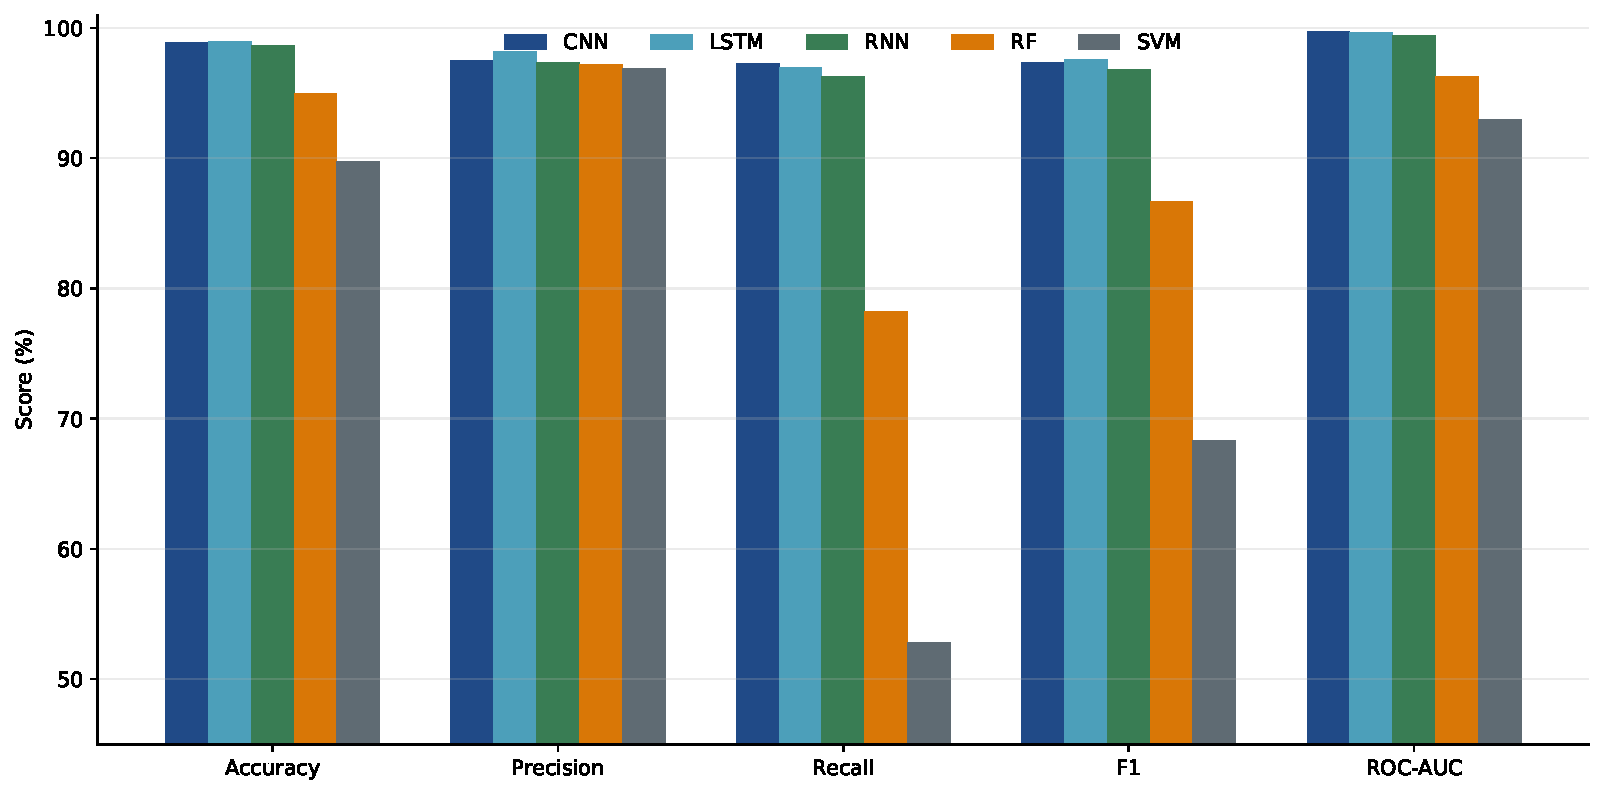
\includegraphics[width=0.98\textwidth]{graphs/v3_baseline_comparison.pdf}
    \caption{Comparison of the Version 3 real-only baseline classifiers.}
    \label{fig:v3-baseline-comparison}
\end{figure}

LSTM obtained the highest internal F1-score and accuracy, while CNN produced
the highest recall and ROC-AUC. RF and especially SVM produced high precision
but missed substantially more phishing URLs. This is visible in their FNRs of
21.78\% and 47.20\%. The result confirms that a high precision value cannot be
used as the only basis for model selection.

These are internal results on a controlled split. They show that the models
learned the registered task, but do not by themselves demonstrate deployment
performance. The external experiments later in this chapter provide the more
difficult generalisation test.

\section{Quality of Generated Phishing URLs}

\subsection{Initial generator comparison}

Each initial GAN produced 500,000 candidate strings. Quality was measured
before downstream classifier training. The main checks were uniqueness,
parse-validity, strict acceptance, overlap with real data, lexical similarity,
coverage of real-data clusters, and difficulty for frozen classifiers.

\begin{table}[htbp]
\centering
\caption{Quality comparison of the initial Version 3 generators.}
\label{tab:initial-gan-quality}
\small
\resizebox{\textwidth}{!}{%
\begin{tabular}{@{}lrrrrrrr@{}}
\toprule
GAN & Unique & Parse-valid & Strictly accepted & Acceptance & Real-cluster coverage & Source AUC & Majority challenging \\
\midrule
SeqGAN  & 99.839\% & 98.171\% & 349,687 & 69.94\% & 94\% & 0.7357 & 10.92\% \\
URL-GAN & 99.806\% & 98.154\% & 239,368 & 47.87\% & 90\% & 0.8817 & 5.06\% \\
RelGAN  & 99.388\% & 81.428\% & 12,869  & 2.57\%  & 86\% & 0.9888 & 0.085\% \\
\bottomrule
\end{tabular}}
\end{table}

\begin{figure}[htbp]
    \centering
    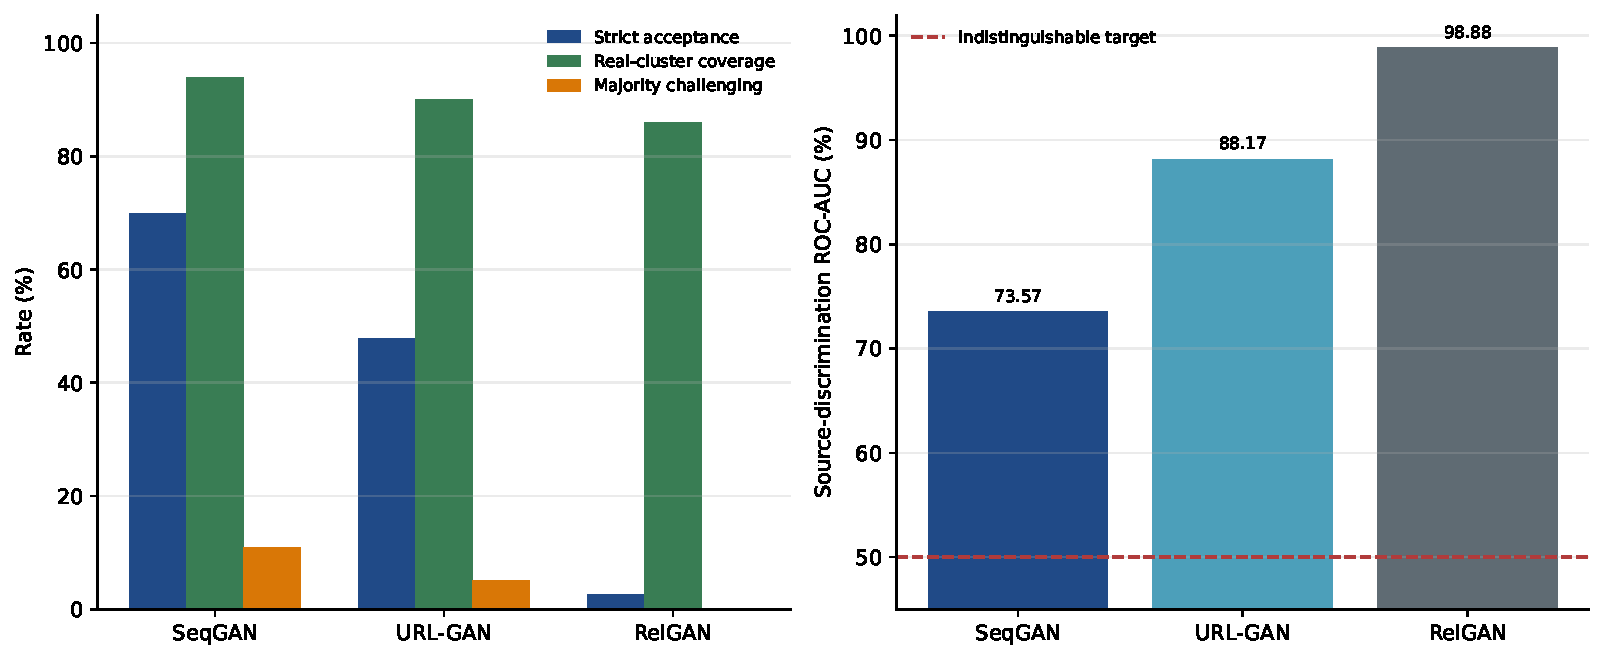
\includegraphics[width=0.97\textwidth]{graphs/gan_quality_comparison.pdf}
    \caption{Generated-URL quality measures for SeqGAN, URL-GAN, and RelGAN.}
    \label{fig:initial-gan-quality}
\end{figure}

All three generators had high raw uniqueness and zero exact memorisation in
the accepted comparison. However, RelGAN's strict acceptance was only 2.57\%.
Its source AUC of 0.9888 also showed that generated and real URLs were easily
distinguished. This demonstrates why uniqueness alone is not sufficient:
malformed or unrealistic strings can still be unique. SeqGAN gave the best
combination of acceptance, real-cluster coverage, lexical closeness, and
classifier challenge, and was therefore the strongest initial generator.

\subsection{MS-HardGAN-C quality}

MS-HardGAN-C was developed after the initial comparison to include source and
structure conditions and a controlled classifier-challenge signal. From
630,000 raw candidates, 309,208 passed the complete acceptance procedure.

\begin{table}[htbp]
\centering
\caption{MS-HardGAN-C generation and filtering results.}
\label{tab:hardgan-quality}
\small
\begin{tabular}{@{}p{0.29\textwidth}p{0.16\textwidth}p{0.45\textwidth}@{}}
\toprule
Measure & Result & Interpretation \\
\midrule
Raw uniqueness & 99.93\% & Candidate duplication was rare. \\
Raw URL-like validity & 94.47\% & Most candidates had a recognisable URL structure before strict filtering. \\
Strictly accepted & 309,208 (49.08\%) & About half passed every registered filter. \\
Accepted uniqueness and validity & 100\% and 100\% & The final pool contained only unique accepted samples. \\
Real URL/hostname overlap & 0 & No accepted sample exactly matched permitted real URLs or hosts. \\
Real-cluster coverage & 90.00\% & The pool represented most registered real lexical clusters. \\
Source ROC-AUC & $0.7992\pm0.0055$ & Real and generated samples remained distinguishable, but not trivially so. \\
Majority challenging & 9.95\% & About one tenth challenged a majority of frozen classifier families. \\
At least one classifier challenging & 52.83\% & More than half challenged at least one family. \\
\bottomrule
\end{tabular}
\end{table}

\begin{figure}[htbp]
    \centering
    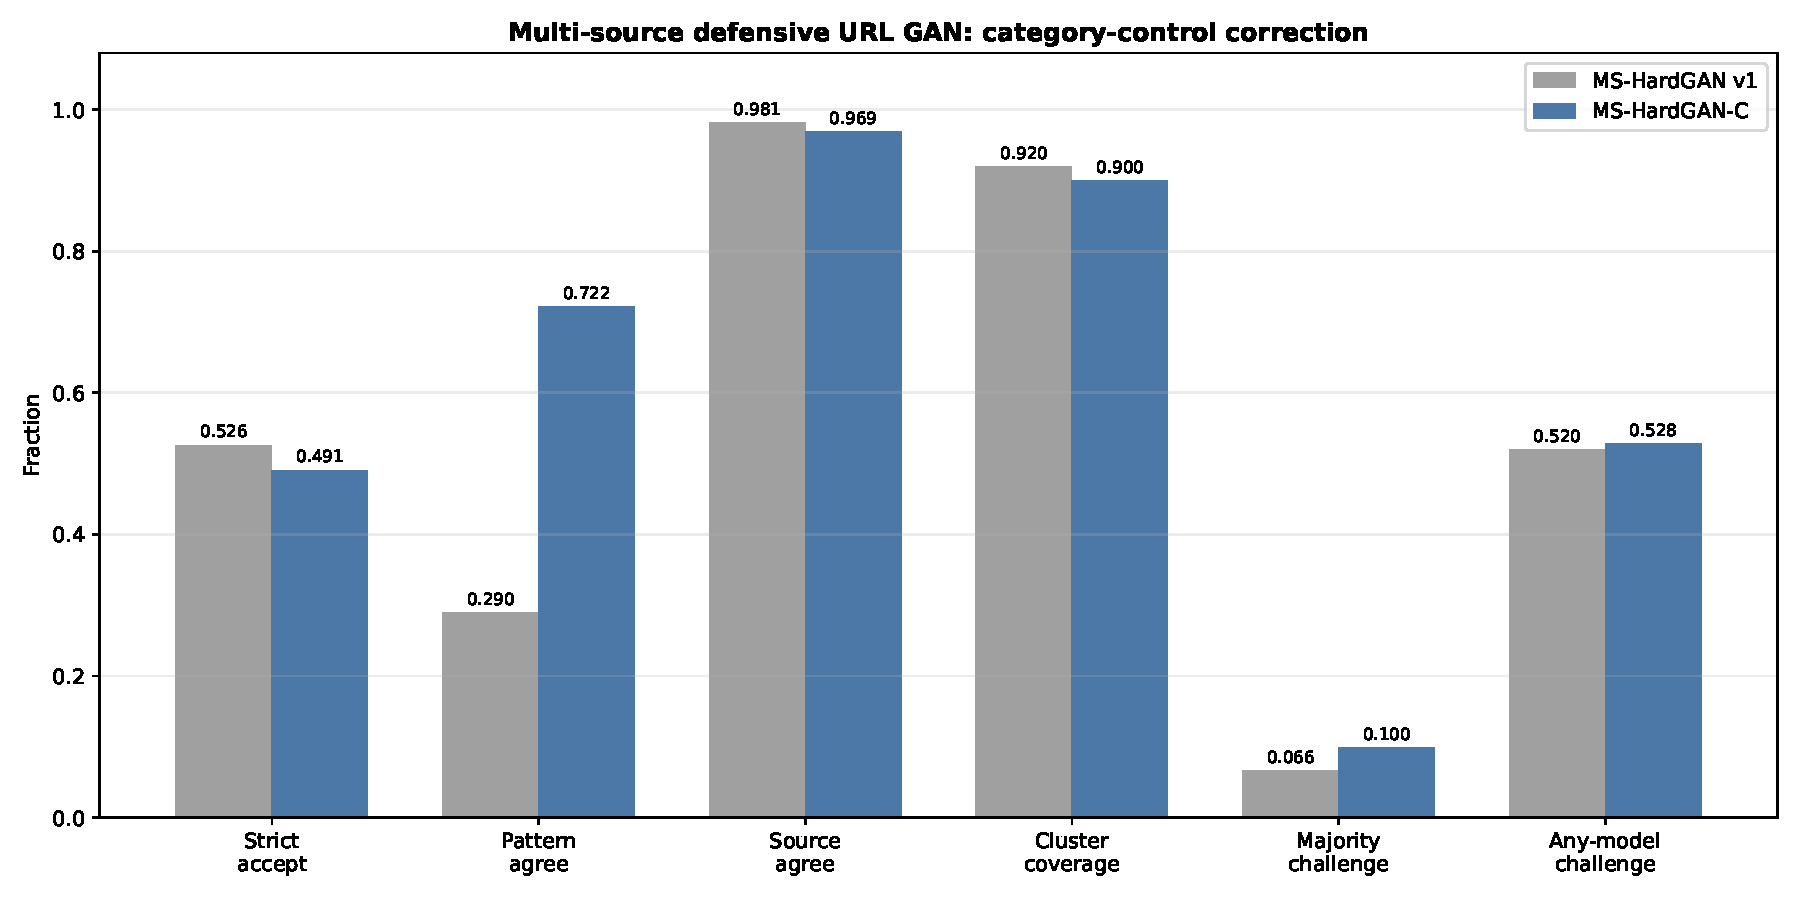
\includegraphics[width=0.97\textwidth]{graphs/ms_hardgan_comparison.pdf}
    \caption{Quality profile of the accepted MS-HardGAN-C URL pool.}
    \label{fig:hardgan-quality}
\end{figure}

The quality tests support using this pool for augmentation experiments, not
claiming that it represents unknown future attacks. The generator recombines
patterns learned from known phishing data and can create difficult, novel
stress examples. It cannot foresee an attack pattern for which there is no
related evidence in the training distribution.

\section{Controlled Augmentation Results}

\subsection{SeqGAN augmentation of the baselines}

The first Version~3 augmentation experiment retained all 358,619 real training
URLs and tested synthetic shares of 10\%, 20\%, 30\%, and 40\%. The table below
reports F1-score because it summarises precision and recall; the complete
multi-metric comparison is shown in Figure~\ref{fig:seqgan-internal}.

\begin{table}[htbp]
\centering
\caption{Internal F1-score under SeqGAN augmentation (mean of three seeds).}
\label{tab:seqgan-f1}
\begin{tabular}{@{}lrrrrr@{}}
\toprule
Model & Real-only & 10\% & 20\% & 30\% & 40\% \\
\midrule
CNN  & 0.9736 & \textbf{0.9764} & 0.9758 & 0.9751 & 0.9724 \\
LSTM & \textbf{0.9756} & 0.9722 & 0.9744 & 0.9750 & 0.9731 \\
RNN  & \textbf{0.9679} & 0.9679 & 0.9532 & 0.9639 & 0.9623 \\
RF   & \textbf{0.8667} & 0.8625 & 0.8576 & 0.8508 & 0.8433 \\
SVM  & 0.6835 & 0.6924 & \textbf{0.6935} & 0.6920 & 0.6887 \\
\bottomrule
\end{tabular}
\end{table}

\begin{figure}[htbp]
    \centering
    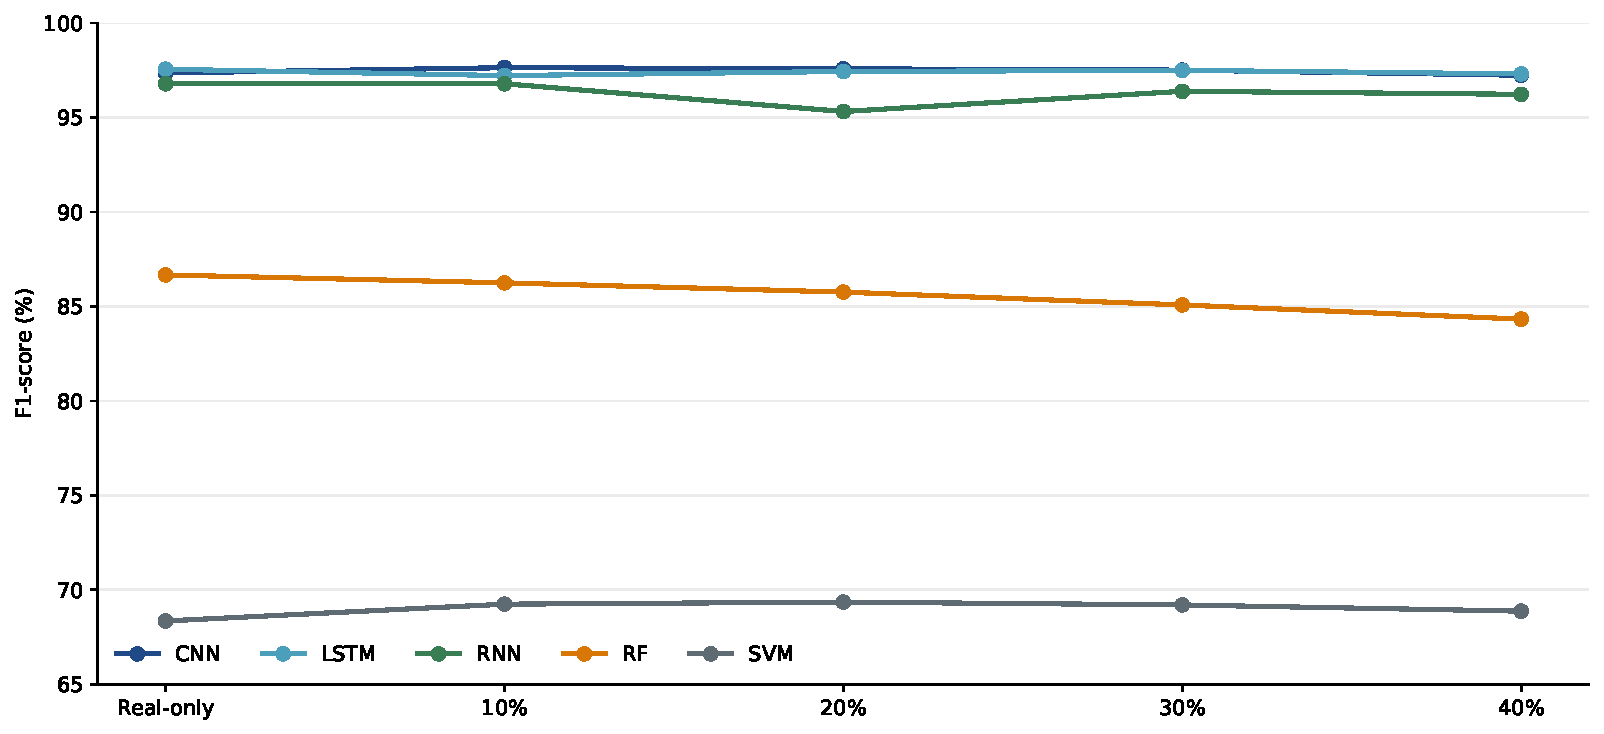
\includegraphics[width=0.98\textwidth]{graphs/seqgan_internal_metrics.pdf}
    \caption{Internal multi-metric results for the SeqGAN augmentation ratios.}
    \label{fig:seqgan-internal}
\end{figure}

SeqGAN produced small, model-specific gains: CNN was strongest at 10\% and SVM
at 20\%. The improvement did not hold across all classifiers. LSTM and RF were
strongest without augmentation, and higher synthetic ratios generally reduced
internal F1. The correct conclusion is therefore not that more synthetic data
is always better, but that its effect depends on the model and synthetic share.

\subsection{MS-HardGAN-C augmentation}

The multi-source experiment used 363,692 fixed real URLs and nested synthetic
pools of 40,410, 90,923, 155,868, and 242,461 URLs. On the unchanged real
internal test set, real-only training remained strongest overall. For example,
CNN F1 decreased from 0.9737 to 0.9728 at 10\%, then to 0.9655 at 40\%.

\begin{figure}[htbp]
    \centering
    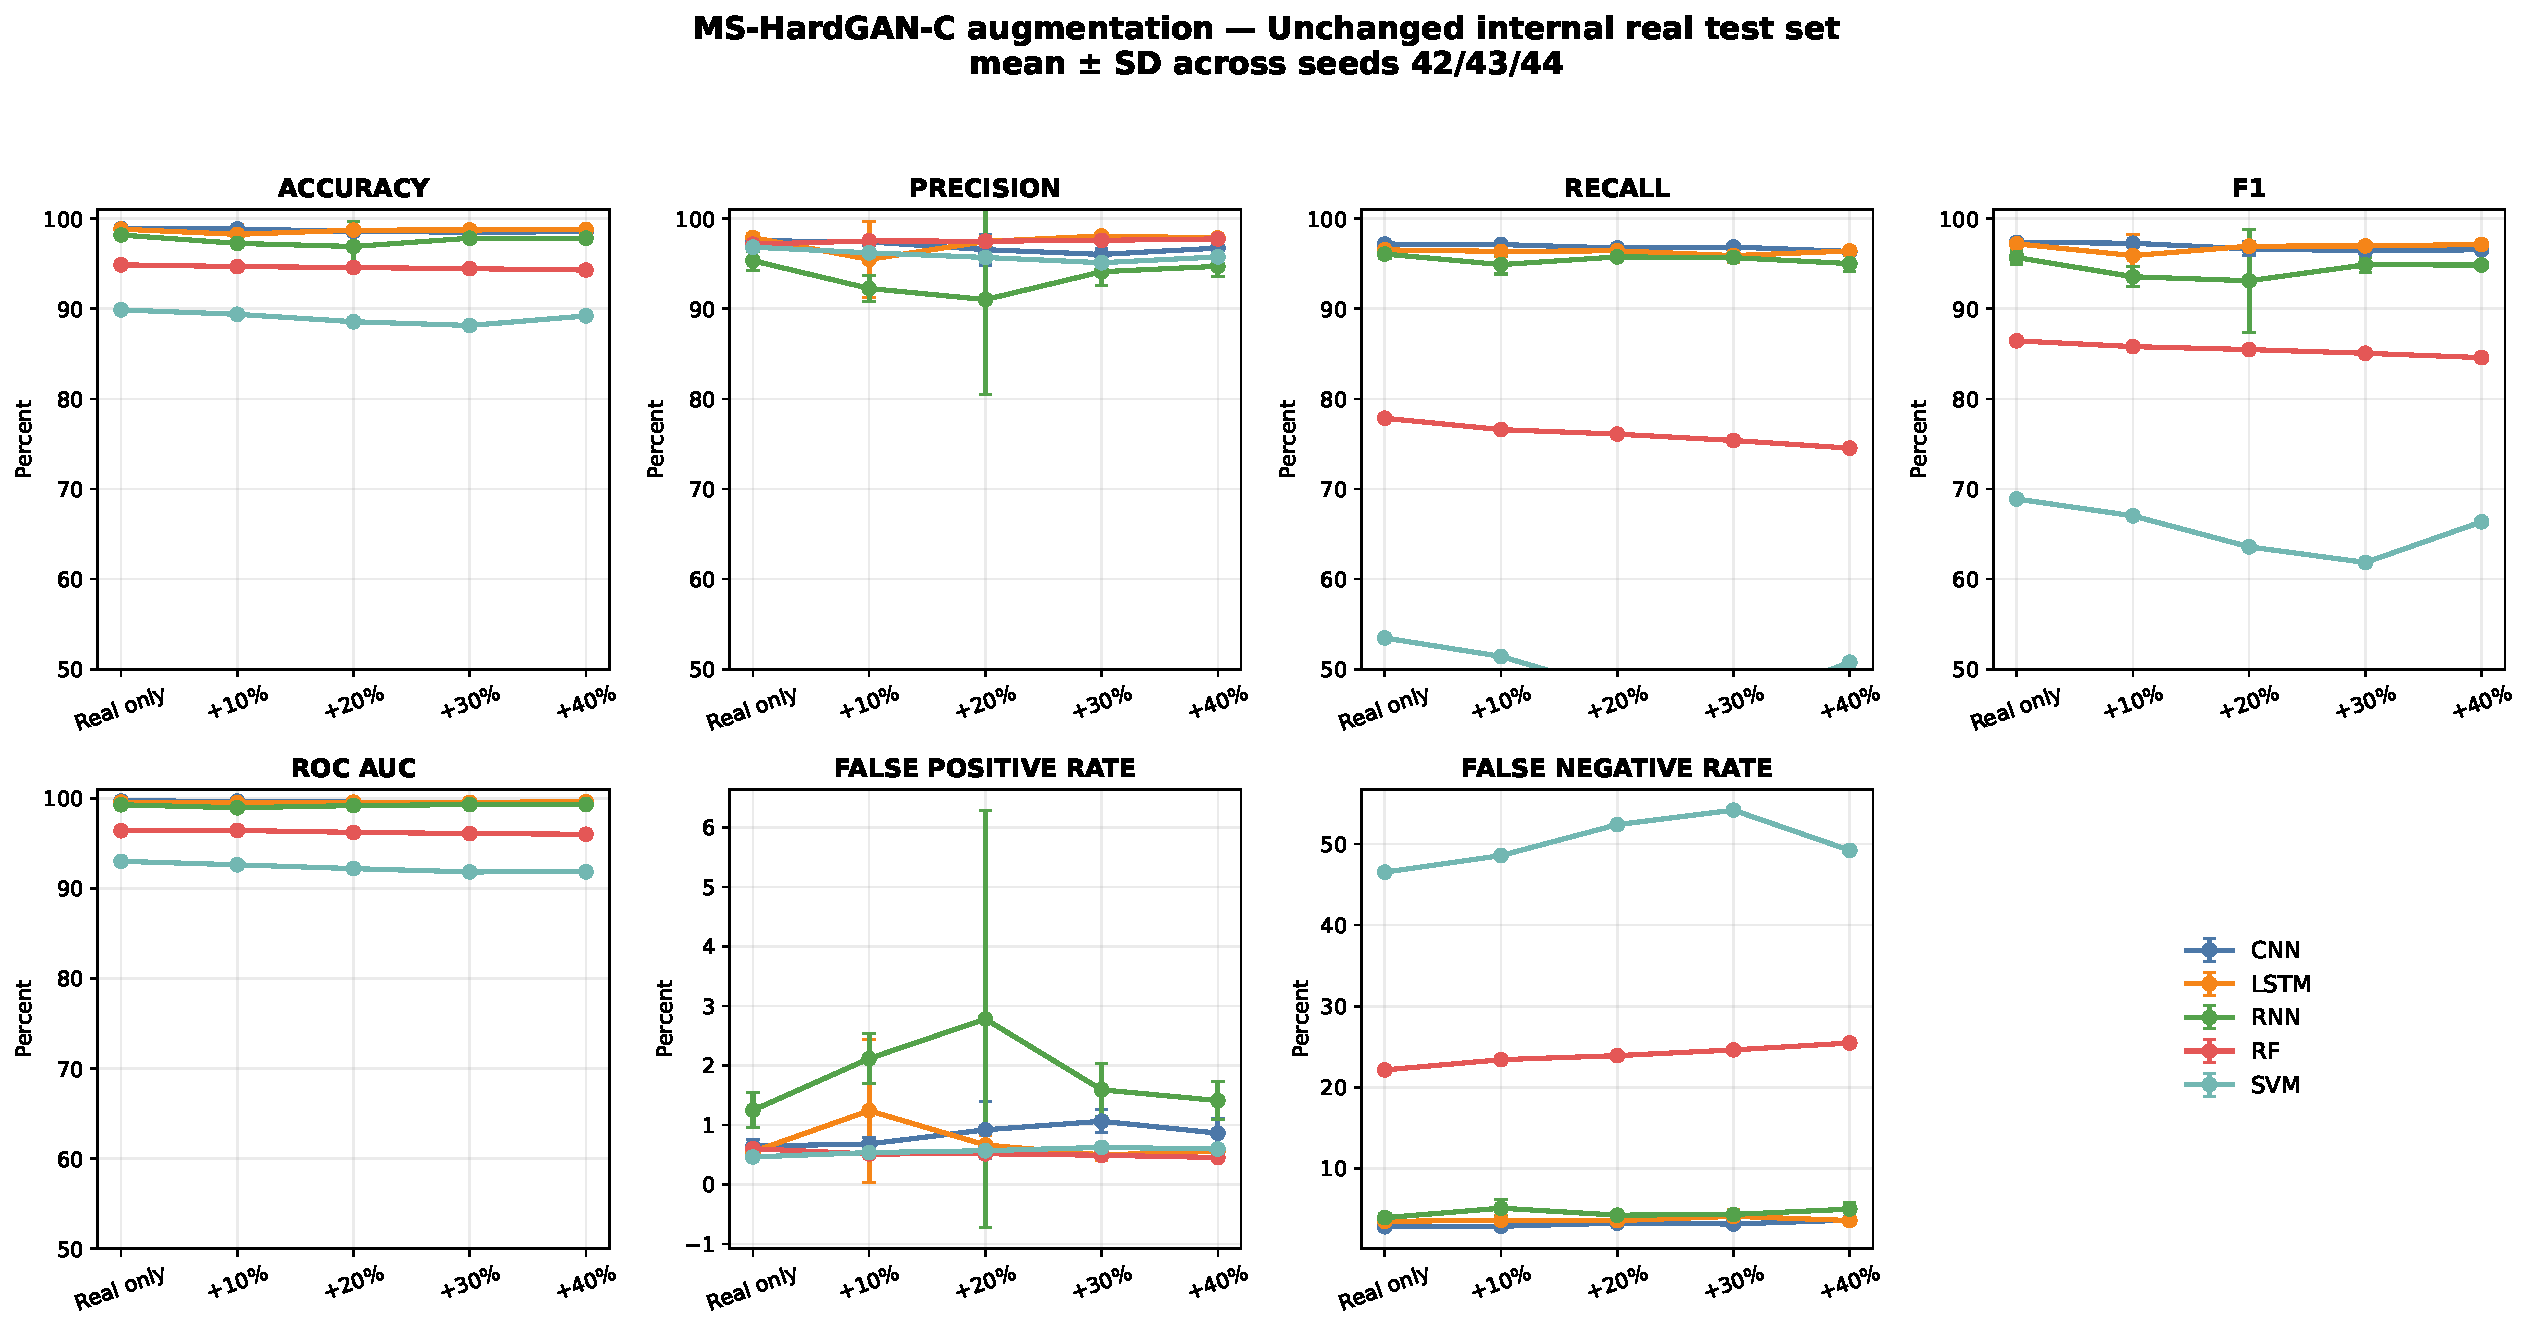
\includegraphics[width=0.98\textwidth]{graphs/ms_hardgan_internal_metrics.pdf}
    \caption{Internal real-test results under MS-HardGAN-C augmentation.}
    \label{fig:hardgan-internal}
\end{figure}

The separate 61,728-row synthetic challenge set gives a different view. It was
held out from both training and synthetic selection. All model families gained
challenge recall at one or more ratios, as shown in
Figure~\ref{fig:hardgan-challenge}. CNN increased from 94.36\% real-only recall
to 98.20\% at 10\%, while LSTM increased from 90.57\% to 97.38\%. RF increased
from 75.78\% to 84.53\%. These gains show stronger recognition of held-out
generator-related patterns, but do not replace evaluation on real URLs.

\begin{figure}[htbp]
    \centering
    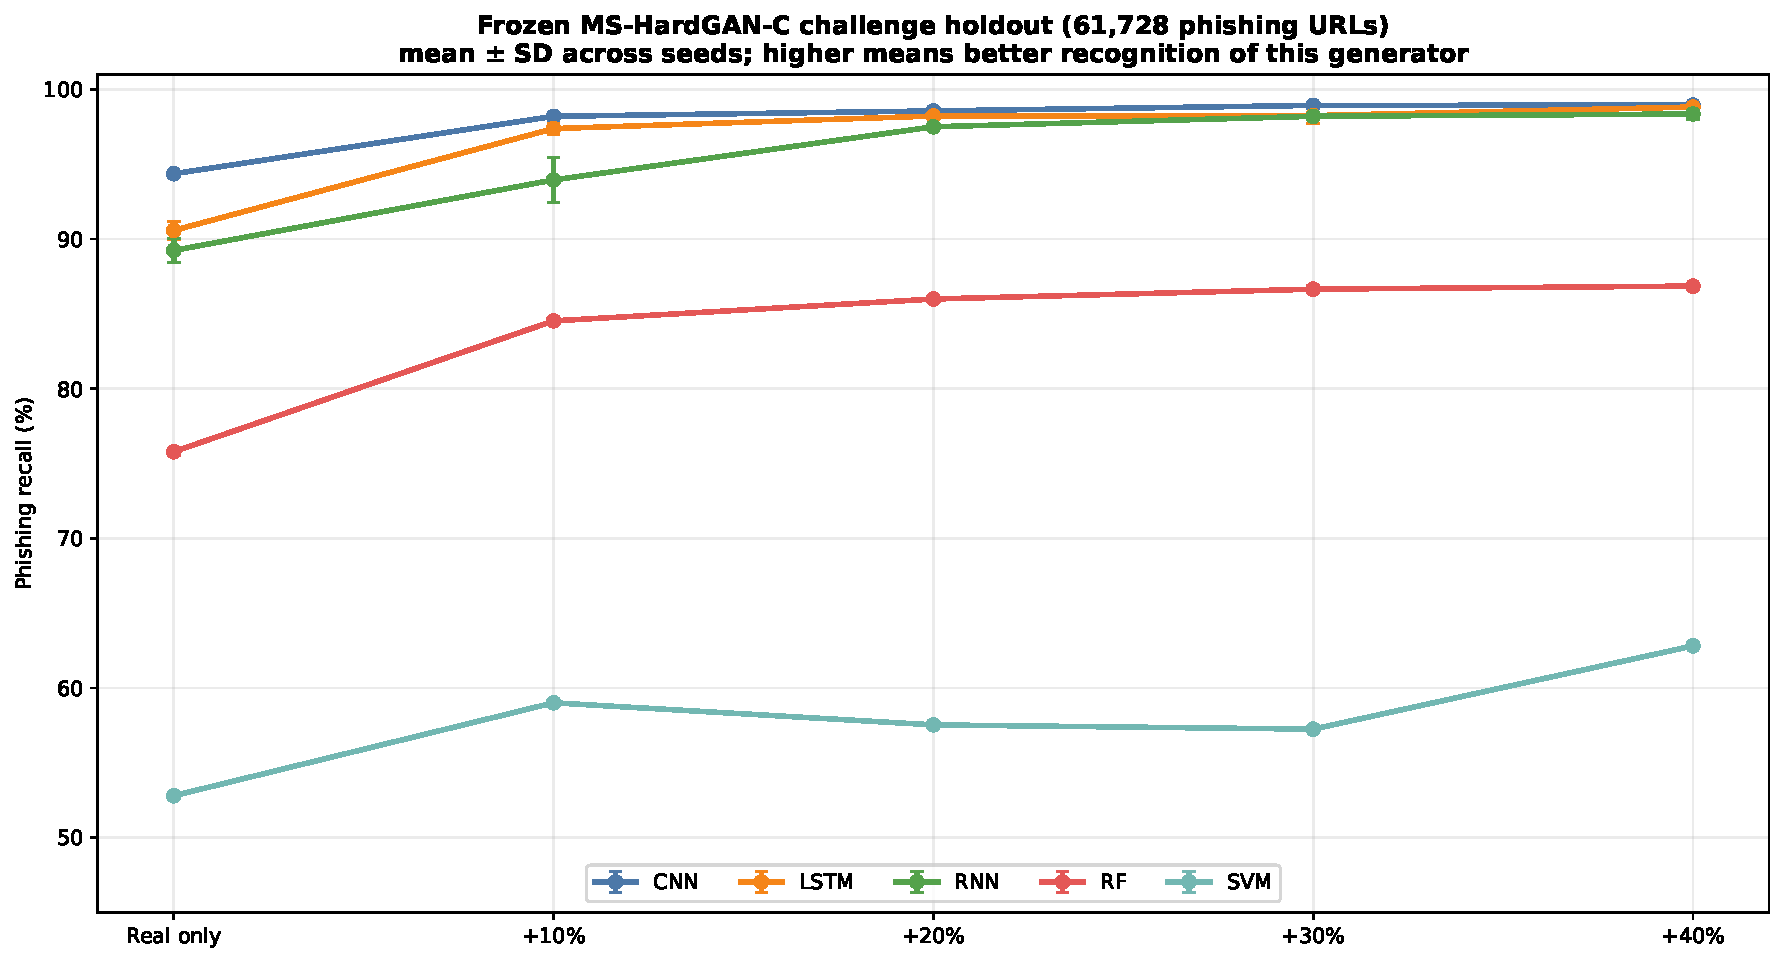
\includegraphics[width=0.97\textwidth]{graphs/ms_hardgan_challenge_recall.pdf}
    \caption{Recall on the frozen MS-HardGAN-C synthetic challenge set.}
    \label{fig:hardgan-challenge}
\end{figure}

Taken together, the internal real and synthetic challenge results answer an
important question. Lower real-test performance after augmentation does not
mean that the classifier failed to learn the generated URLs. In this case the
opposite occurred: synthetic-challenge recall increased while performance on
the real distribution sometimes decreased. The evidence points to a
distribution trade-off rather than simple failure to classify GAN samples.

\subsection{Matched SeqGAN and MS-HardGAN-C comparison}
\label{sec:matched-generator-comparison}

The earlier SeqGAN and MS-HardGAN-C studies had different development roles
and did not use exactly the same phishing input. To remove this input-data
confound, SeqGAN was retrained on the exact 84,280 phishing rows used by
MS-HardGAN-C. The matched SeqGAN generated 500,000 candidates, of which
344,507 passed strict filtering. Exactly 40,410 clean URLs were added to the
same 363,692 real HYB-MS rows used by the MS-HardGAN-C 10\% condition.

Both augmented conditions used the same HYB-MS architecture, weighted sampler,
features, seeds 42/43/44, and frozen evaluation rows. Each three-seed ensemble
selected its threshold using the same separate 400-row calibration cohort,
maximising calibration F1 subject to calibration FPR no greater than 1\%.
Neither external set was used for threshold selection. The external 30K set in
Table~\ref{tab:matched-generator-results} contains 30.07\% phishing and is
different from the later primary 30K low-prevalence test.

\begin{table}[htbp]
\centering
\caption{Matched-input generator comparison using the same HYB-MS procedure (\%).}
\label{tab:matched-generator-results}
\scriptsize
\resizebox{\textwidth}{!}{%
\begin{tabular}{@{}llrrrrrrrr@{}}
\toprule
Dataset & Condition & Accuracy & Precision & Recall & F1 & ROC-AUC & PR-AUC & FPR & FNR \\
\midrule
Internal & Real-only & 96.08 & 99.95 & 81.35 & 89.70 & 99.64 & 99.23 & 0.01 & 18.65 \\
 & SeqGAN 10\% & 96.24 & 99.93 & 82.13 & 90.16 & \textbf{99.72} & \textbf{99.35} & 0.02 & 17.87 \\
 & MS-HardGAN-C 10\% & \textbf{96.45} & 99.93 & \textbf{83.13} & \textbf{90.76} & 99.55 & 99.09 & 0.02 & \textbf{16.87} \\
\midrule
External 10K & Real-only & 91.77 & 98.04 & 85.24 & 91.20 & 96.63 & 97.53 & 1.70 & 14.76 \\
 & SeqGAN 10\% & 92.14 & 98.44 & 85.64 & 91.59 & 96.60 & 97.57 & 1.36 & 14.36 \\
 & MS-HardGAN-C 10\% & \textbf{93.08} & \textbf{98.47} & \textbf{87.52} & \textbf{92.67} & \textbf{96.90} & \textbf{97.84} & 1.36 & \textbf{12.48} \\
\midrule
External 30K & Real-only & 94.64 & 96.54 & 85.25 & 90.54 & 96.95 & 96.05 & 1.32 & 14.75 \\
 & SeqGAN 10\% & 94.53 & 97.02 & 84.41 & 90.28 & 96.70 & 95.85 & 1.12 & 15.59 \\
 & MS-HardGAN-C 10\% & \textbf{95.42} & \textbf{97.53} & \textbf{86.99} & \textbf{91.96} & \textbf{97.00} & \textbf{96.41} & \textbf{0.95} & \textbf{13.01} \\
\bottomrule
\end{tabular}}
\end{table}

\begin{figure}[htbp]
    \centering
    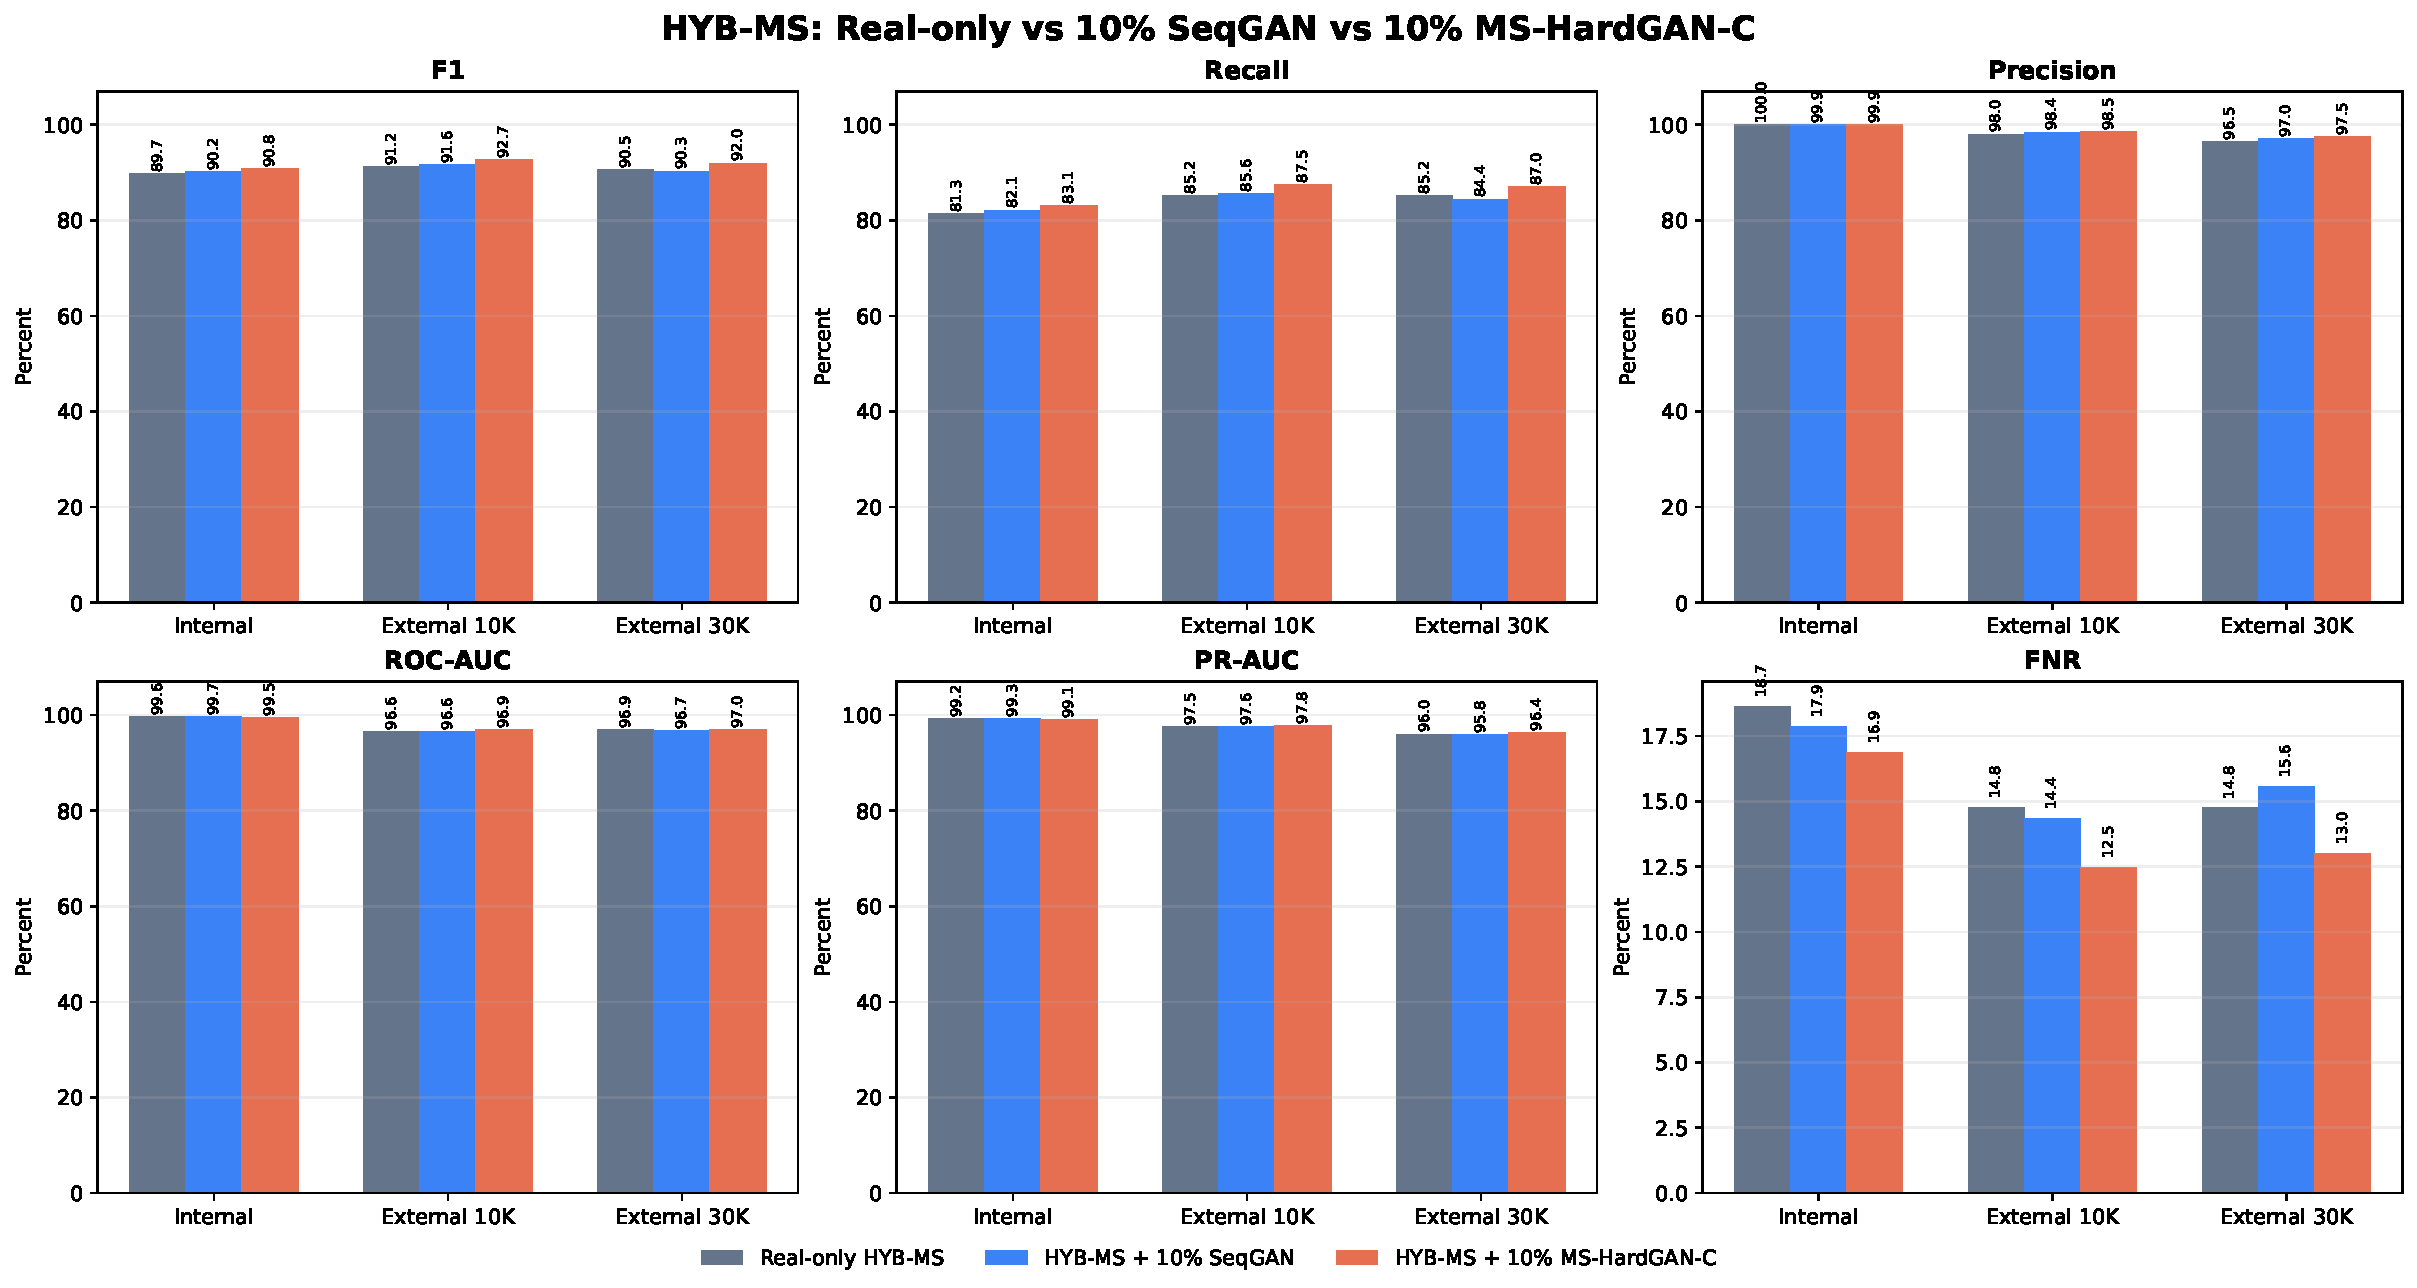
\includegraphics[width=\textwidth]{graphs/hybrid_generator_matched_comparison.pdf}
    \caption{Real-only HYB-MS and the two matched-input 10\% generator conditions.}
    \label{fig:matched-generator-comparison}
\end{figure}

Matching the phishing input substantially improved SeqGAN's downstream result.
On the external 10K set, its F1 increased from 88.54\% in the earlier unmatched
comparison to 91.59\%, and FNR fell from 20.14\% to 14.36\%. This confirms that
generator training data was an important confound. MS-HardGAN-C nevertheless
remained stronger after the confound was removed. At the same 1.36\% external
10K FPR, it increased recall by 1.88 points and reduced FNR by 1.88 points
relative to matched SeqGAN. On the external 30K set it also achieved higher
F1, higher recall, lower FPR, and lower FNR. The result supports choosing
MS-HardGAN-C for HYB-MS because its conditional structural, source, and
classifier-challenge objectives produced a more useful augmentation pool, not
because it had access to additional real phishing identities.

\subsection{Final hybrid ratio comparison}

The final HYB-MS comparison used the same hybrid architecture for the real-only
and GAN-augmented conditions. The real rows, seeds, test rows, and evaluation
rules were fixed. A balanced 10,000-row external set was used to compare the
augmentation ratios with separately calibrated ensemble thresholds.

\begin{table}[htbp]
\centering
\caption{Calibrated HYB-MS results on the frozen balanced 10K external set (\%).}
\label{tab:hybrid-10k-ratios}
\small
\resizebox{\textwidth}{!}{%
\begin{tabular}{@{}lrrrrrrrr@{}}
\toprule
Condition & Accuracy & Precision & Recall & F1 & ROC-AUC & PR-AUC & FPR & FNR \\
\midrule
Real-only & 91.77 & 98.04 & 85.24 & 91.20 & 96.63 & 97.49 & 1.70 & 14.76 \\
GAN 10\%  & \textbf{93.10} & 98.43 & \textbf{87.60} & \textbf{92.70} & \textbf{96.89} & \textbf{97.81} & 1.40 & \textbf{12.40} \\
GAN 20\%  & 91.30 & 98.96 & 83.48 & 90.56 & 96.30 & 97.44 & 0.88 & 16.52 \\
GAN 30\%  & 88.39 & 99.23 & 77.38 & 86.95 & 95.85 & 96.91 & 0.60 & 22.62 \\
GAN 40\%  & 85.15 & \textbf{99.30} & 70.80 & 82.66 & 95.55 & 96.64 & \textbf{0.50} & 29.20 \\
\bottomrule
\end{tabular}}
\end{table}

The 10\% condition gave the best balanced result. Larger ratios reduced FPR and
raised precision, but the cost was a sharp loss of phishing recall. Therefore,
10\% was retained as the main augmentation condition; it was not selected by
changing the tested ratios after the final results were observed.

\section{External Evaluation}

\subsection{Why prevalence matters}

A balanced test is useful for comparing classes, but browser traffic normally
contains many more legitimate than phishing URLs. In a low-prevalence setting,
even a small FPR can produce many false warnings, while accuracy can appear
high simply because most rows are legitimate. Later external snapshots
therefore used phishing shares of approximately 5\% and 3\%, and results are
reported with confusion-derived FPR and FNR.

\subsection{External comparison of classifier families}

The hybrid was not chosen only because it was the most complex model. A final
equal-calibration comparison applied the same calibration data, threshold rule,
balanced 10K and 30K external sets, and eligibility checks to the competing
model families. Table~\ref{tab:external-classifiers} reports the balanced 10K
results. The ordinary multi-source baselines and real-only HYB-MS used the same
363,692 stored real URL identities. HYB-MS additionally used its declared
weighted source-sampling and class-conditional alignment procedure; these are
part of the model design rather than extra unique training URLs.

\begin{table}[htbp]
\centering
\caption{Equal-calibration external comparison on the balanced 10K set (\%).}
\label{tab:external-classifiers}
\small
\resizebox{\textwidth}{!}{%
\begin{tabular}{@{}lrrrrrrrr@{}}
\toprule
Model & Accuracy & Precision & Recall & F1 & ROC-AUC & PR-AUC & FPR & FNR \\
\midrule
CNN-MS & 55.47 & 95.51 & 11.48 & 20.50 & 79.83 & 81.12 & \textbf{0.54} & 88.52 \\
LSTM-MS & 90.63 & 98.54 & 82.48 & 89.80 & 93.72 & 96.08 & 1.22 & 17.52 \\
RNN-MS & 66.79 & 96.66 & 34.78 & 51.15 & 89.01 & 91.29 & 1.20 & 65.22 \\
RF-MS & 65.13 & 96.04 & 31.56 & 47.51 & 63.01 & 74.37 & 1.30 & 68.44 \\
SVM-MS & 52.95 & 86.78 & 6.96 & 12.89 & 24.99 & 43.72 & 1.06 & 93.04 \\
HYB-MS real-only & 91.77 & 98.04 & 85.24 & 91.20 & 96.63 & 97.49 & 1.70 & 14.76 \\
HYB-MS +10\% & \textbf{93.10} & 98.43 & \textbf{87.60} & \textbf{92.70} & \textbf{96.89} & \textbf{97.81} & 1.40 & \textbf{12.40} \\
\bottomrule
\end{tabular}}
\end{table}

\begin{figure}[htbp]
    \centering
    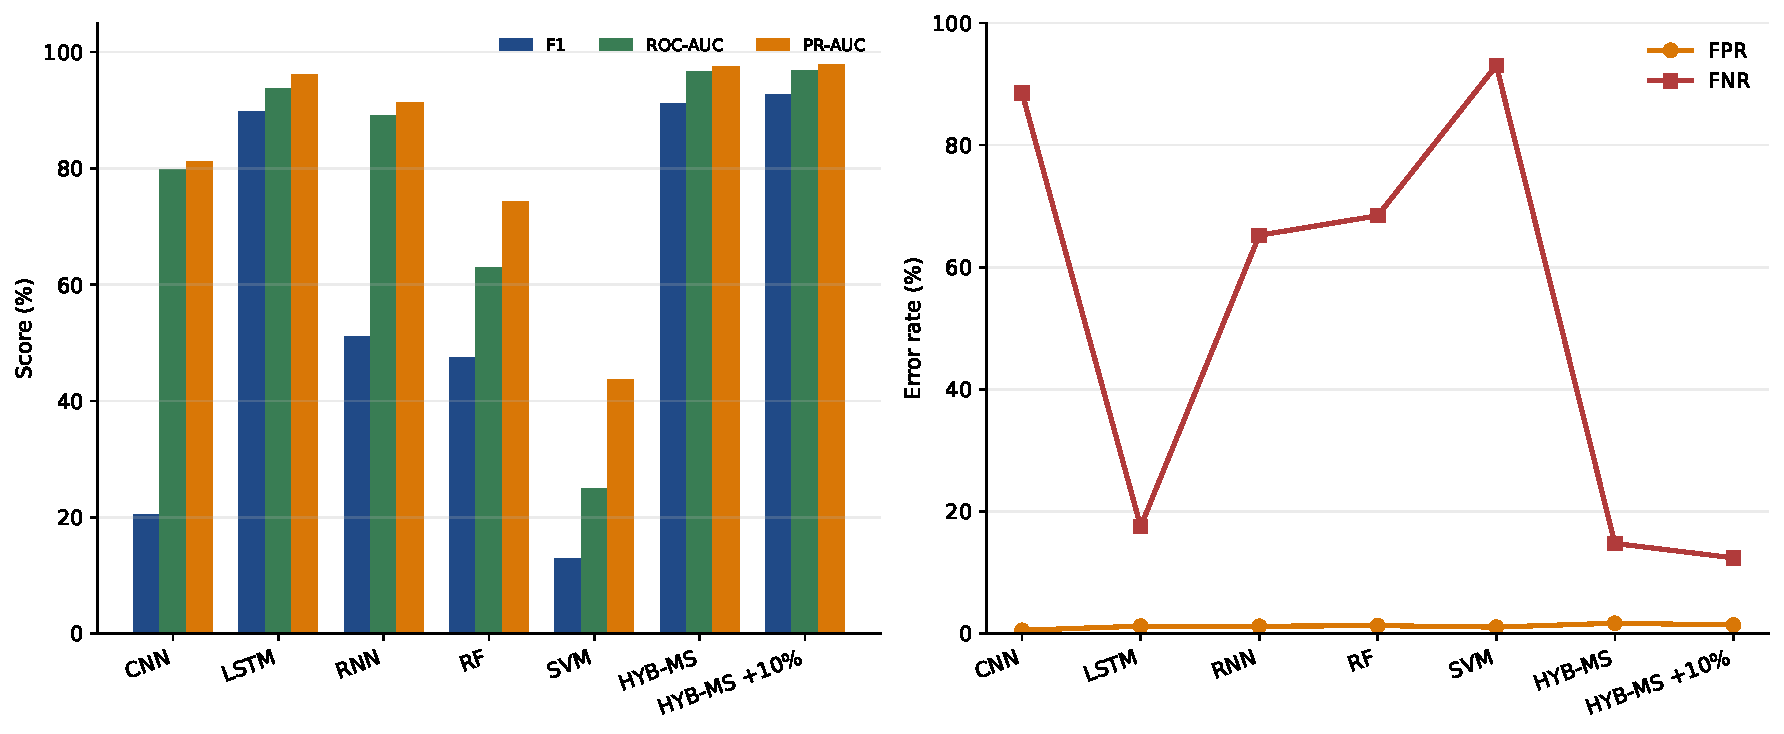
\includegraphics[width=0.99\textwidth]{graphs/external_classifier_comparison.pdf}
    \caption{External performance of the equally calibrated classifier families.}
    \label{fig:external-classifier-comparison}
\end{figure}

LSTM-MS was the strongest non-hybrid external baseline, with F1 89.80\%.
Real-only HYB-MS improved F1 to 91.20\%, ROC-AUC to 96.63\%, and FNR to
14.76\%. The 10\% GAN-augmented hybrid then produced the strongest external F1
and the lowest FNR among the eligible high-performing models. Although CNN-MS
had the lowest FPR, it detected only 11.48\% of phishing URLs; that operating
point was not a useful security balance.

The hybrid was consequently selected for three connected reasons. First, its
character CNN learns local spelling and delimiter patterns, while the lexical
branch retains full-URL structural evidence, including information beyond the
128-character sequence limit. Second, weighted source exposure and
class-conditional alignment were introduced specifically to reduce the source
shift identified in Version~2. Third, the equal-calibration results show that
these design choices improved external F1 and reduced missed phishing relative
to the strongest ordinary baseline. The GAN contribution was then measured
fairly by comparing HYB-MS real-only and HYB-MS +10\%, which have the same
architecture and differ only in the registered synthetic training rows.

\subsection{Primary 30K low-prevalence confirmation}

The frozen 30,000-row evaluation contained 28,500 legitimate and 1,500 phishing
URLs. The five ordinary multi-source baselines, HYB-MS real-only, and HYB-MS
with 10\% augmentation were evaluated on these same rows. All checkpoints and
equal-calibration thresholds remained frozen; no model was retrained or tuned
for this comparison.

\begin{table}[htbp]
\centering
\caption{All classifier results on the 30K external set with 5\% phishing prevalence.}
\label{tab:external-30k}
\small
\resizebox{\textwidth}{!}{%
\begin{tabular}{@{}lrrrrrrrr@{}}
\toprule
Model & Accuracy & Precision & Recall & F1 & ROC-AUC & PR-AUC & FPR & FNR \\
\midrule
CNN-MS & 95.31\% & 66.32\% & 12.60\% & 21.18\% & 79.95\% & 31.81\% & \textbf{0.34\%} & 87.40\% \\
LSTM-MS & 97.48\% & 74.65\% & 75.20\% & 74.93\% & 92.61\% & 81.70\% & 1.34\% & 24.80\% \\
RNN-MS & 96.16\% & 68.64\% & 42.60\% & 52.57\% & 88.46\% & 58.53\% & 1.02\% & 57.40\% \\
RF-MS & 95.13\% & 52.70\% & 25.40\% & 34.28\% & 53.56\% & 30.71\% & 1.20\% & 74.60\% \\
SVM-MS & 94.33\% & 26.74\% & 7.67\% & 11.92\% & 28.11\% & 8.28\% & 1.11\% & 92.33\% \\
HYB-MS real-only & 97.85\% & 77.16\% & 81.07\% & 79.06\% & 96.58\% & 84.29\% & 1.26\% & 18.93\% \\
HYB-MS +10\% & \textbf{98.12\%} & \textbf{80.95\%} & \textbf{81.60\%} & \textbf{81.27\%} & \textbf{96.82\%} & \textbf{87.27\%} & 1.01\% & \textbf{18.40\%} \\
\bottomrule
\end{tabular}}
\end{table}

\begin{figure}[htbp]
    \centering
    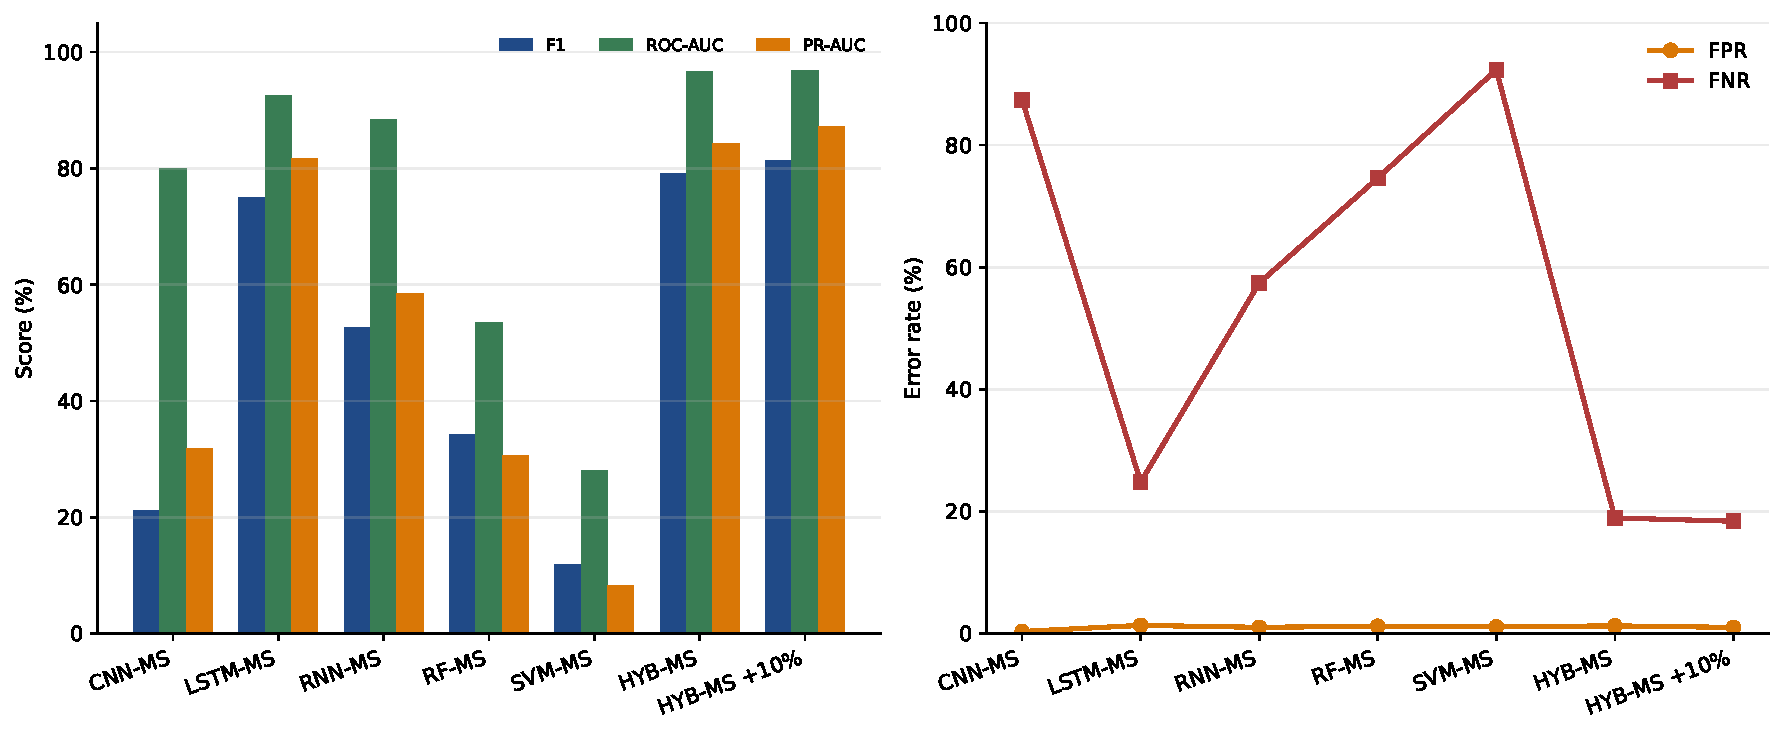
\includegraphics[width=0.99\textwidth]{graphs/final_30k_all_classifiers.pdf}
    \caption{All classifiers on the frozen 30K low-prevalence external set.}
    \label{fig:external-30k-classifiers}
\end{figure}

LSTM-MS was again the strongest ordinary baseline, reaching 74.93\% F1 and
75.20\% recall. HYB-MS real-only improved these values to 79.06\% F1 and
81.07\% recall. HYB-MS +10\% produced the strongest overall result: 81.27\%
F1, 81.60\% recall, 96.82\% ROC-AUC, and 87.27\% PR-AUC. CNN-MS achieved the
smallest FPR, but its 12.60\% recall meant that it missed most phishing URLs;
this was not an acceptable balance. The common dataset and frozen thresholds
therefore provide direct external evidence for selecting the hybrid rather
than selecting it only from its internal performance.

The 10\% model produced 288 false positives and 276 false negatives, compared
with 360 and 284 for real-only. McNemar's paired test over all changed decisions
gave $p=7.43\times10^{-5}$. The bootstrap 95\% confidence interval for the F1
change was approximately +1.05 to +3.41 percentage points, while the recall
change alone was not significant on the phishing subset ($p=0.526$). The most
defensible statement is that 10\% augmentation improved the overall decision
balance and reduced false positives on this snapshot; evidence for a standalone
recall improvement was weaker.

\subsection{Independent PhishTank and later frozen snapshots}

Additional snapshots tested whether the result repeated when the phishing
source or prevalence changed. The PhishTank-only evaluation used verified
PhishTank phishing URLs \citep{phishtankdeveloper}. Legitimate rows were kept
substantially more numerous than phishing rows in every low-prevalence test.

\begin{table}[htbp]
\centering
\caption{External comparison of real-only and 10\% GAN-augmented HYB-MS (\%).}
\label{tab:external-summary}
\small
\resizebox{\textwidth}{!}{%
\begin{tabular}{@{}llrrrrrr@{}}
\toprule
Dataset & Condition & Accuracy & Precision & Recall & F1 & FPR & FNR \\
\midrule
PhishTank 10K, 5\% & Real-only & 98.00 & 76.88 & 85.80 & 81.10 & 1.36 & 14.20 \\
 & GAN 10\% & \textbf{98.45} & \textbf{81.89} & \textbf{88.60} & \textbf{85.11} & \textbf{1.03} & \textbf{11.40} \\
Final labelled 6K, 5\% & Real-only & 97.95 & 82.18 & 75.33 & 78.61 & 0.86 & 24.67 \\
 & GAN 10\% & \textbf{98.23} & \textbf{84.15} & \textbf{79.67} & \textbf{81.85} & \textbf{0.79} & \textbf{20.33} \\
Post-freeze 10K, 3\% & Real-only & 98.71 & 77.14 & 81.00 & 79.02 & 0.74 & 19.00 \\
 & GAN 10\% & \textbf{98.80} & \textbf{78.48} & \textbf{82.67} & \textbf{80.52} & \textbf{0.70} & \textbf{17.33} \\
\bottomrule
\end{tabular}}
\end{table}

\begin{figure}[htbp]
    \centering
    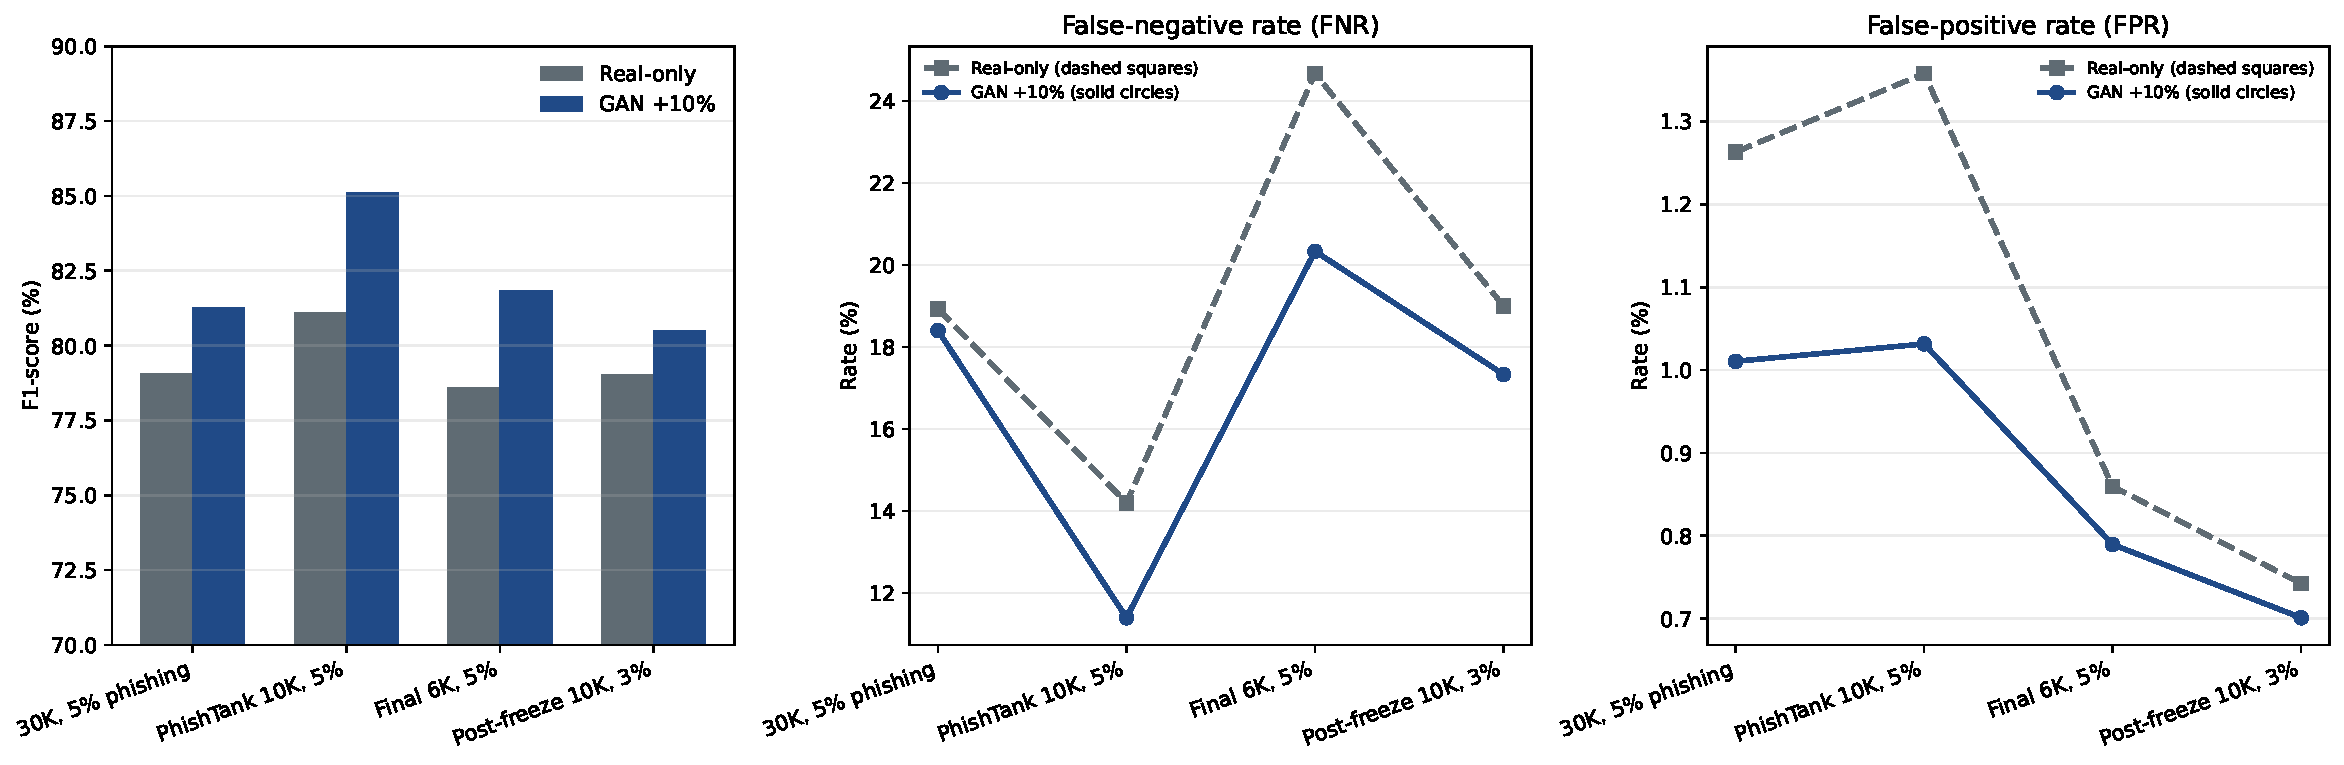
\includegraphics[width=0.99\textwidth]{graphs/external_real_only_vs_gan10.pdf}
    \caption{F1, FPR, and FNR across the low-prevalence external evaluations. Grey dashed lines with square markers represent the real-only model; blue solid lines with circular markers represent the 10\% GAN-augmented model.}
    \label{fig:external-summary}
\end{figure}

The 10\% condition improved F1 and reduced both FPR and FNR in all four listed
low-prevalence snapshots, including the 30K result in
Table~\ref{tab:external-30k}. The size of the gain varied, so it should be
reported as repeated empirical improvement under these test conditions rather
than proof that augmentation will improve every future dataset.

\subsection{Long-URL stress test}

Long legitimate URLs were deliberately included in a separate stress test
because earlier browser observations showed that length could contribute to
false warnings. This set was a targeted diagnostic and not a representative
estimate of ordinary traffic.

\begin{table}[htbp]
\centering
\caption{Results on the long-URL stress set (\%).}
\label{tab:long-url-stress}
\begin{tabular}{@{}lrrrrrrr@{}}
\toprule
Condition & Accuracy & Precision & Recall & F1 & ROC-AUC & FPR & FNR \\
\midrule
Real-only & 96.95 & 88.00 & 77.00 & 82.13 & 98.51 & 1.05 & 23.00 \\
GAN 10\%  & 96.86 & 84.66 & 80.00 & 82.26 & 98.42 & 1.45 & 20.00 \\
\bottomrule
\end{tabular}
\end{table}

GAN augmentation detected six additional phishing URLs but introduced eight
additional false positives. F1 changed only slightly and the predeclared
directional non-regression check was not passed. Consequently, long URLs remain
a stated limitation. They should not be treated as phishing solely because of
length; the full combination of character and lexical evidence is required.

\section{Threshold Analysis}

The model produces a continuous score, while a threshold converts the score to
a class decision. Lower thresholds classify more URLs as phishing. This reduces
FNR but usually increases FPR and can reduce precision, especially when real
phishing prevalence is low. Thresholds were selected using calibration data,
not the final test labels.

\begin{table}[htbp]
\centering
\caption{Single-stage threshold policies on the registered threshold evaluation set.}
\label{tab:threshold-policies}
\small
\resizebox{\textwidth}{!}{%
\begin{tabular}{@{}lrrrrrr@{}}
\toprule
Policy & Threshold & Precision & Recall & F1 & FPR & FNR \\
\midrule
Ultra-strict & 0.999973 & 99.37\% & 31.60\% & 47.95\% & 0.02\% & 68.40\% \\
Strict & 0.999849 & 98.60\% & 45.75\% & 62.50\% & 0.07\% & 54.25\% \\
Conservative & 0.995319 & 94.83\% & 79.85\% & 86.70\% & 0.48\% & 20.15\% \\
Balanced & 0.970766 & 89.77\% & 87.35\% & 88.55\% & 1.11\% & 12.65\% \\
Recall-first & 0.885636 & 81.57\% & 90.75\% & 85.92\% & 2.28\% & 9.25\% \\
High-recall & 0.670915 & 64.84\% & 93.60\% & 76.61\% & 5.64\% & 6.40\% \\
\bottomrule
\end{tabular}}
\end{table}

\begin{figure}[htbp]
    \centering
    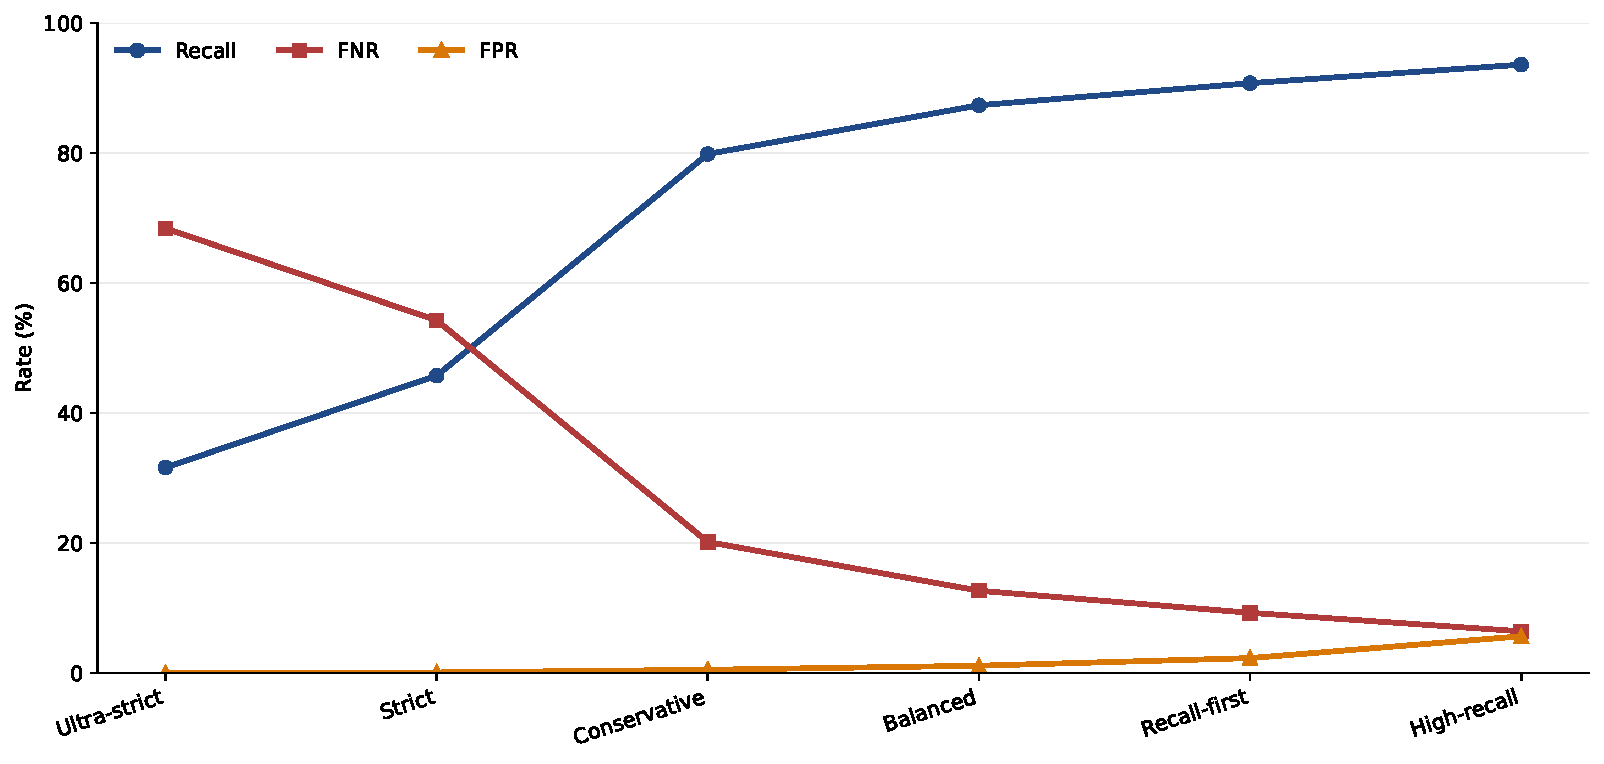
\includegraphics[width=0.98\textwidth]{graphs/threshold_tradeoff.pdf}
    \caption{Recall, FPR, and FNR trade-off across the registered score policies.}
    \label{fig:threshold-tradeoff}
\end{figure}

The high-recall threshold reduced FNR to 6.40\%, but raised FPR to 5.64\%. In a
stream containing thousands of legitimate pages, this would create too many
warnings. Conversely, the strict thresholds achieved very low FPR but missed
more than half of phishing URLs. The balanced region provides a more practical
starting point, while a browser can use score bands so that moderate evidence
creates a caution rather than an immediate block. The implementation of those
warning modes is discussed in Chapter~7.

\section{Discussion of the Research Questions}

\subsection{Can a URL-only classifier detect phishing effectively?}

Yes, within the evaluated distributions. CNN and LSTM achieved internal F1
above 97\%, and the hybrid models produced useful discrimination on multiple
external sets. However, external FNR was consistently higher than internal FNR.
URL-only detection is therefore useful as a defensive signal, not a guarantee
that every phishing page will be identified.

\subsection{Does GAN augmentation improve detection?}

This research question was investigated experimentally; it did not begin with
the assumption that augmentation must improve every metric or every model.
Random and high-ratio augmentation produced mixed results and sometimes reduced
performance on the internal real test set. This negative evidence is part of
the answer because it shows that the quantity and quality of generated URLs
matter.

The controlled 10\% MS-HardGAN-C condition gave the clearest positive result.
Using the same hybrid architecture, real identities, seeds, calibration method,
and test rows, it improved F1 and the confusion-matrix balance on several frozen
low-prevalence external datasets. On the primary 30K set it also outperformed
all five ordinary classifier families. The study therefore finds that carefully
filtered GAN augmentation \emph{can} improve URL-phishing detection under the
evaluated conditions. This directly answers the research question while
recognising that the observed benefit depends on the generator, augmentation
ratio, classifier, and evaluation distribution.

The matched-input generator ablation strengthens this interpretation. After
SeqGAN and MS-HardGAN-C were trained on the exact same 84,280 phishing rows,
both 10\% pools improved HYB-MS on the balanced external 10K set, but
MS-HardGAN-C retained the higher F1 and lower FNR. Thus, its advantage cannot
be explained only by its earlier access to 2,061 additional multi-source
phishing rows.

\subsection{Are the generated URLs useful beyond final accuracy?}

Yes. The generators produced large novel pools with no exact accepted overlap
with the permitted real URLs. Held-out synthetic-challenge recall increased
substantially after augmentation, showing that the added samples expanded
coverage of difficult generator-related patterns. The realism and source-AUC
tests also identified poor generators that raw uniqueness would have accepted.
These quality results are an independent contribution even where downstream
real-test metrics did not improve.

\subsection{What remains difficult?}

Distribution shift remains the main limitation. Source-specific structure,
long legitimate URLs, new phishing campaigns, and changing class prevalence
all alter the error balance. Threshold lowering can reduce FNR, but it cannot
eliminate missed phishing without increasing false warnings. Continued testing
on later data is therefore necessary for any operational use.

\section{Chapter Summary}

The experiments established strong internal neural baselines, compared four
implemented GAN designs using quality measures beyond uniqueness, and tested
augmentation without forcing a positive outcome. SeqGAN was the strongest
initial generator. When SeqGAN was later retrained on the same 84,280 phishing
rows as MS-HardGAN-C, its HYB-MS augmentation result improved, but
MS-HardGAN-C still supplied the stronger 10\% pool. High augmentation ratios were generally harmful to real-test balance,
whereas the 10\% hybrid condition produced the most consistent external gains.

The results also showed that metric interpretation depends on prevalence and
threshold choice. A reduction in FNR can be purchased at the cost of many false
positives, and high accuracy can conceal weak phishing recall. Chapter~7 now
examines how these findings were translated into browser warning behaviour and
how the extension performed during technical and user evaluation.
